\documentclass{standalone}
\usepackage{tikz}
\usetikzlibrary{patterns, positioning}
\usepackage[sfdefault]{ClearSans} %% option 'sfdefault' activates Clear Sans as the default text font
\usepackage[T1]{fontenc}

\begin{document}
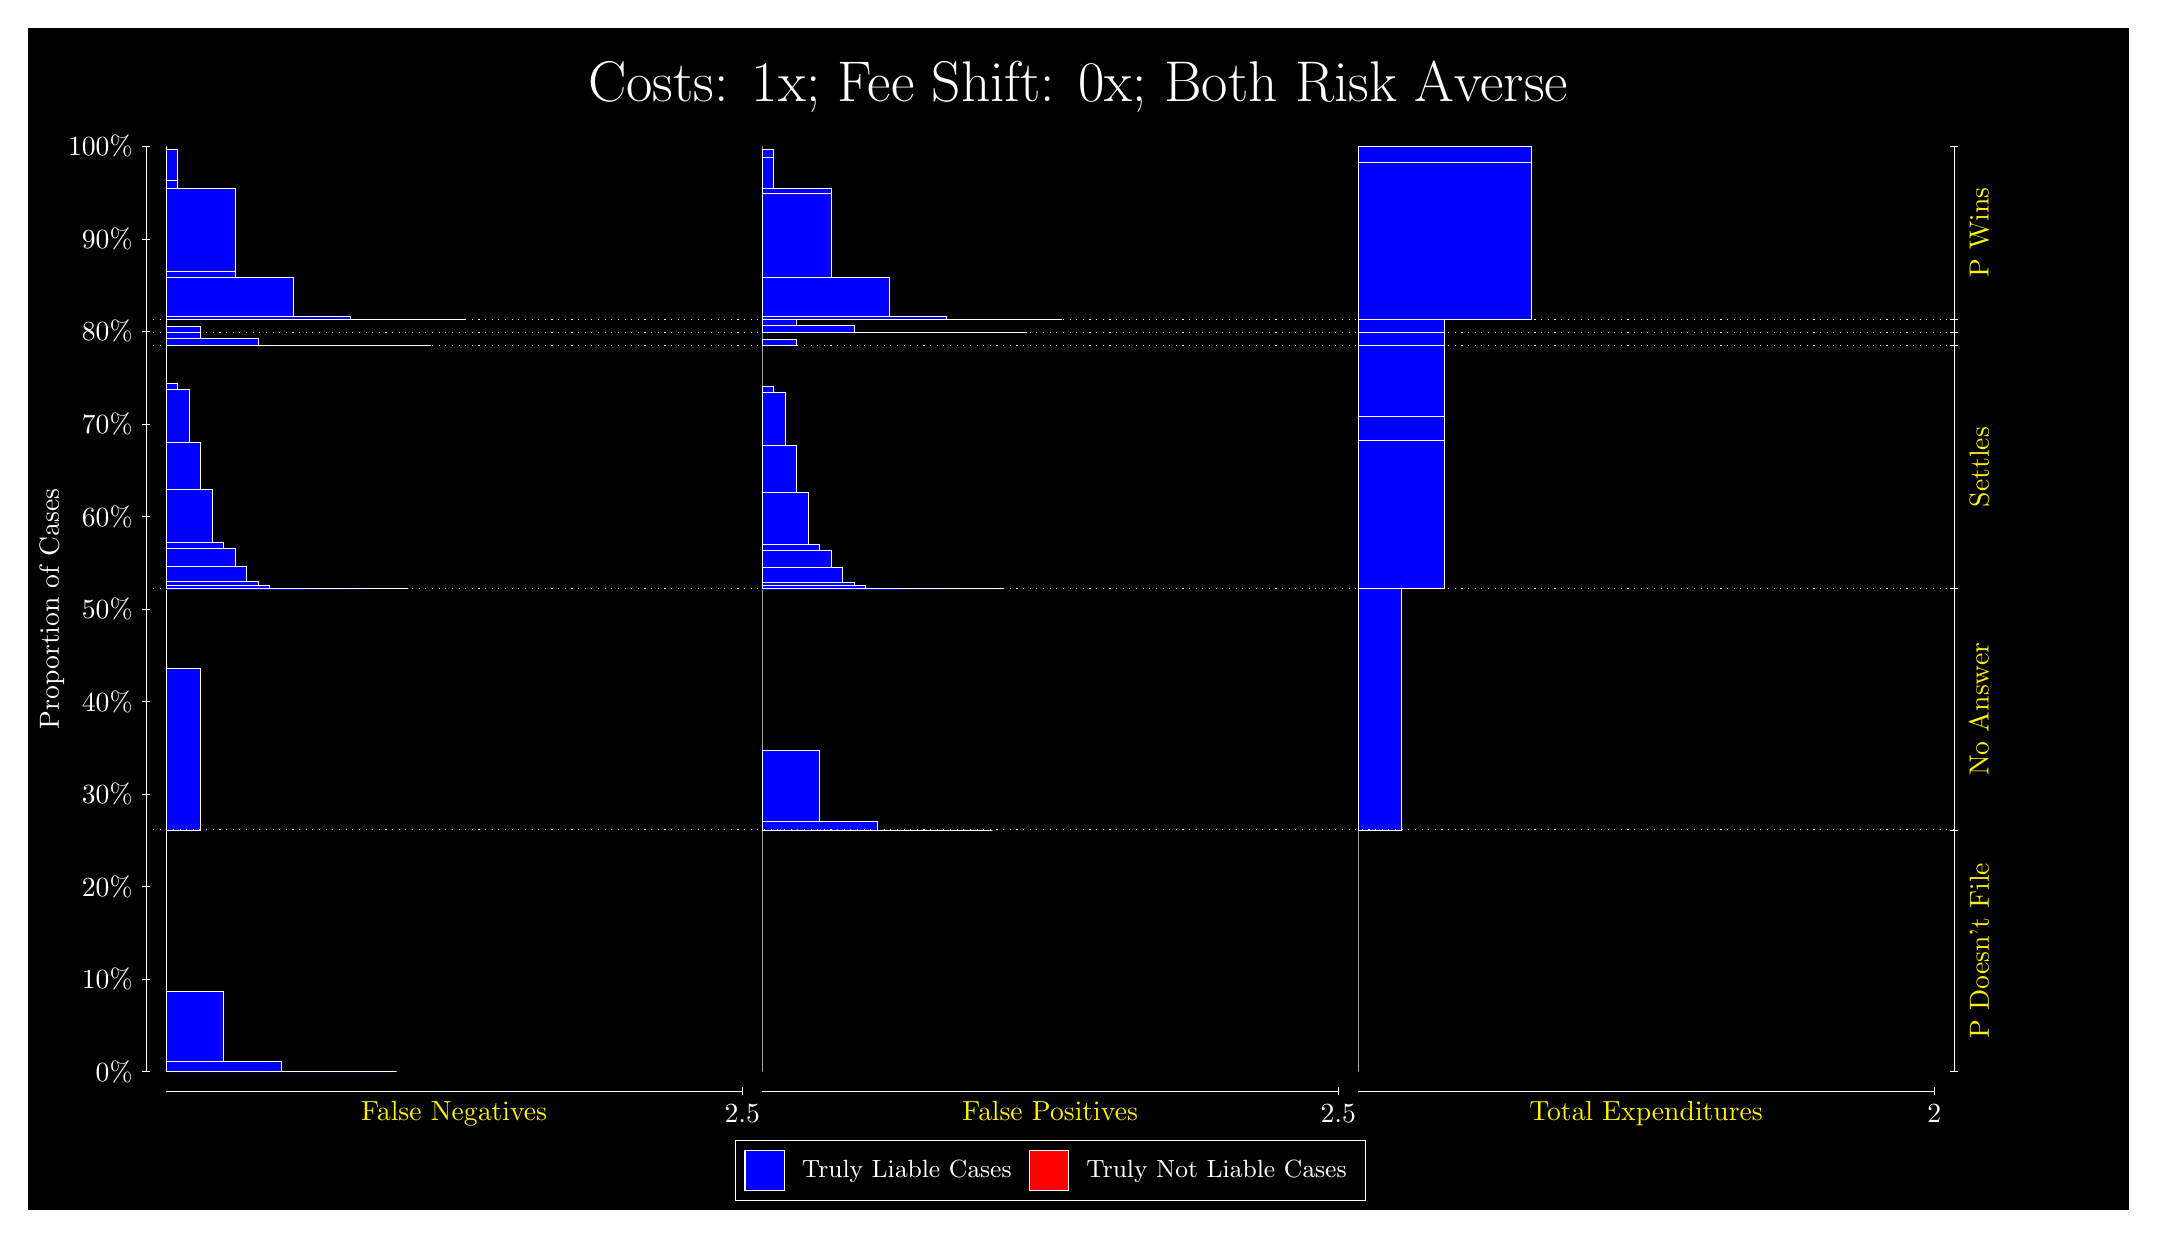
\begin{tikzpicture}
\draw[fill=black] (0,0) rectangle (26.667,15);
\draw[text=white] (0,13.5) rectangle (26.667,15) node[midway] {\huge Costs: 1x; Fee Shift: 0x; Both Risk Averse};
\draw[white, very thin] (1.5,1.75) -- (1.5,13.5);
\node[rotate=90, text=white, anchor=center] at (0.3, 7.625) {Proportion of Cases};
\draw[white, very thin] (1.45,1.75) -- (1.55,1.75);
\node[text=white, anchor=east] at (1.45, 1.75) {0\%};
\draw[white, very thin] (1.45,2.925) -- (1.55,2.925);
\node[text=white, anchor=east] at (1.45, 2.925) {10\%};
\draw[white, very thin] (1.45,4.1) -- (1.55,4.1);
\node[text=white, anchor=east] at (1.45, 4.1) {20\%};
\draw[white, very thin] (1.45,5.275) -- (1.55,5.275);
\node[text=white, anchor=east] at (1.45, 5.275) {30\%};
\draw[white, very thin] (1.45,6.45) -- (1.55,6.45);
\node[text=white, anchor=east] at (1.45, 6.45) {40\%};
\draw[white, very thin] (1.45,7.625) -- (1.55,7.625);
\node[text=white, anchor=east] at (1.45, 7.625) {50\%};
\draw[white, very thin] (1.45,8.8) -- (1.55,8.8);
\node[text=white, anchor=east] at (1.45, 8.8) {60\%};
\draw[white, very thin] (1.45,9.975) -- (1.55,9.975);
\node[text=white, anchor=east] at (1.45, 9.975) {70\%};
\draw[white, very thin] (1.45,11.15) -- (1.55,11.15);
\node[text=white, anchor=east] at (1.45, 11.15) {80\%};
\draw[white, very thin] (1.45,12.325) -- (1.55,12.325);
\node[text=white, anchor=east] at (1.45, 12.325) {90\%};
\draw[white, very thin] (1.45,13.5) -- (1.55,13.5);
\node[text=white, anchor=east] at (1.45, 13.5) {100\%};

\draw[white, very thin] (24.457,1.75) -- (24.457,13.5);
\draw[white, very thin] (24.407,1.75) -- (24.507,1.75);
\node[anchor=west] at (24.407, 1.75) {};
\draw[white, very thin] (24.407,4.8182) -- (24.507,4.8182);
\node[anchor=west] at (24.407, 4.8182) {};
\draw[white, very thin] (24.407,7.882) -- (24.507,7.882);
\node[anchor=west] at (24.407, 7.882) {};
\draw[white, very thin] (24.407,10.971) -- (24.507,10.971);
\node[anchor=west] at (24.407, 10.971) {};
\draw[white, very thin] (24.407,11.138) -- (24.507,11.138);
\node[anchor=west] at (24.407, 11.138) {};
\draw[white, very thin] (24.407,11.305) -- (24.507,11.305);
\node[anchor=west] at (24.407, 11.305) {};
\draw[white, very thin] (24.407,13.5) -- (24.507,13.5);
\node[anchor=west] at (24.407, 13.5) {};

\draw[white, very thin, fill=blue] (1.75,1.75) rectangle (4.6775,1.75);
\draw[white, very thin, fill=blue] (1.75,1.75) rectangle (3.9457,1.751);
\draw[white, very thin, fill=blue] (1.75,1.751) rectangle (3.2138,1.8747);
\draw[white, very thin, fill=blue] (1.75,1.8747) rectangle (2.4819,2.7682);
\draw[white, very thin, fill=red] (1.75,2.7682) rectangle (1.75,2.7682);
\draw[white, very thin, fill=blue] (1.75,2.7682) rectangle (1.75,4.8182);
\draw[white, very thin, fill=blue] (1.75,4.8182) rectangle (2.1891,6.8699);
\draw[white, very thin, fill=red] (1.75,6.8699) rectangle (1.75,6.8699);
\draw[white, very thin, fill=blue] (1.75,6.8699) rectangle (1.75,7.882);
\draw[white, very thin, fill=blue] (1.75,7.882) rectangle (4.8239,7.882);
\draw[white, very thin, fill=blue] (1.75,7.882) rectangle (4.2384,7.882);
\draw[white, very thin, fill=blue] (1.75,7.882) rectangle (4.092,7.882);
\draw[white, very thin, fill=blue] (1.75,7.882) rectangle (3.6529,7.8821);
\draw[white, very thin, fill=blue] (1.75,7.8821) rectangle (3.5065,7.8824);
\draw[white, very thin, fill=blue] (1.75,7.8824) rectangle (3.3602,7.8922);
\draw[white, very thin, fill=blue] (1.75,7.8922) rectangle (3.0674,7.9305);
\draw[white, very thin, fill=blue] (1.75,7.9305) rectangle (2.921,7.9755);
\draw[white, very thin, fill=blue] (1.75,7.9755) rectangle (2.7746,8.1717);
\draw[white, very thin, fill=blue] (1.75,8.1717) rectangle (2.6283,8.3995);
\draw[white, very thin, fill=blue] (1.75,8.3995) rectangle (2.4819,8.4725);
\draw[white, very thin, fill=blue] (1.75,8.4725) rectangle (2.3355,9.1474);
\draw[white, very thin, fill=blue] (1.75,9.1474) rectangle (2.1891,9.7473);
\draw[white, very thin, fill=blue] (1.75,9.7473) rectangle (2.0428,10.409);
\draw[white, very thin, fill=blue] (1.75,10.409) rectangle (1.8964,10.485);
\draw[white, very thin, fill=red] (1.75,10.485) rectangle (1.75,10.485);
\draw[white, very thin, fill=blue] (1.75,10.485) rectangle (1.75,10.971);
\draw[white, very thin, fill=blue] (1.75,10.971) rectangle (5.1167,10.971);
\draw[white, very thin, fill=blue] (1.75,10.971) rectangle (4.3848,10.971);
\draw[white, very thin, fill=blue] (1.75,10.971) rectangle (3.6529,10.973);
\draw[white, very thin, fill=blue] (1.75,10.973) rectangle (2.921,11.057);
\draw[white, very thin, fill=blue] (1.75,11.057) rectangle (2.1891,11.138);
\draw[white, very thin, fill=red] (1.75,11.138) rectangle (1.75,11.138);
\draw[white, very thin, fill=blue] (1.75,11.138) rectangle (2.1891,11.219);
\draw[white, very thin, fill=red] (1.75,11.219) rectangle (1.75,11.219);
\draw[white, very thin, fill=blue] (1.75,11.219) rectangle (1.75,11.305);
\draw[white, very thin, fill=blue] (1.75,11.305) rectangle (5.5558,11.305);
\draw[white, very thin, fill=blue] (1.75,11.305) rectangle (4.8239,11.306);
\draw[white, very thin, fill=blue] (1.75,11.306) rectangle (4.092,11.343);
\draw[white, very thin, fill=blue] (1.75,11.343) rectangle (3.3602,11.836);
\draw[white, very thin, fill=blue] (1.75,11.836) rectangle (2.6283,11.907);
\draw[white, very thin, fill=blue] (1.75,11.907) rectangle (2.6283,12.969);
\draw[white, very thin, fill=blue] (1.75,12.969) rectangle (1.8964,13.071);
\draw[white, very thin, fill=blue] (1.75,13.071) rectangle (1.8964,13.462);
\draw[white, very thin, fill=red] (1.75,13.462) rectangle (1.75,13.462);
\draw[white, very thin, fill=blue] (1.75,13.462) rectangle (1.75,13.5);
\draw[white, very thin, fill=red] (9.3189,1.75) rectangle (9.3189,1.75);
\draw[white, very thin, fill=blue] (9.3189,1.75) rectangle (9.3189,4.8182);
\draw[white, very thin, fill=red] (9.3189,4.8182) rectangle (12.246,4.8182);
\draw[white, very thin, fill=blue] (9.3189,4.8182) rectangle (12.246,4.8182);
\draw[white, very thin, fill=blue] (9.3189,4.8182) rectangle (11.515,4.8186);
\draw[white, very thin, fill=blue] (9.3189,4.8186) rectangle (10.783,4.9309);
\draw[white, very thin, fill=blue] (9.3189,4.9309) rectangle (10.051,5.8303);
\draw[white, very thin, fill=blue] (9.3189,5.8303) rectangle (9.3189,7.882);
\draw[white, very thin, fill=red] (9.3189,7.882) rectangle (12.393,7.882);
\draw[white, very thin, fill=blue] (9.3189,7.882) rectangle (12.393,7.882);
\draw[white, very thin, fill=red] (9.3189,7.882) rectangle (11.807,7.882);
\draw[white, very thin, fill=blue] (9.3189,7.882) rectangle (11.807,7.882);
\draw[white, very thin, fill=blue] (9.3189,7.882) rectangle (11.661,7.882);
\draw[white, very thin, fill=red] (9.3189,7.882) rectangle (11.222,7.882);
\draw[white, very thin, fill=blue] (9.3189,7.882) rectangle (11.222,7.8821);
\draw[white, very thin, fill=blue] (9.3189,7.8821) rectangle (11.075,7.8824);
\draw[white, very thin, fill=blue] (9.3189,7.8824) rectangle (10.929,7.8912);
\draw[white, very thin, fill=red] (9.3189,7.8912) rectangle (10.636,7.8912);
\draw[white, very thin, fill=blue] (9.3189,7.8912) rectangle (10.636,7.9285);
\draw[white, very thin, fill=blue] (9.3189,7.9285) rectangle (10.49,7.9639);
\draw[white, very thin, fill=blue] (9.3189,7.9639) rectangle (10.344,8.1598);
\draw[white, very thin, fill=blue] (9.3189,8.1598) rectangle (10.197,8.3681);
\draw[white, very thin, fill=red] (9.3189,8.3681) rectangle (10.051,8.3681);
\draw[white, very thin, fill=blue] (9.3189,8.3681) rectangle (10.051,8.444);
\draw[white, very thin, fill=blue] (9.3189,8.444) rectangle (9.9044,9.1058);
\draw[white, very thin, fill=blue] (9.3189,9.1058) rectangle (9.758,9.7057);
\draw[white, very thin, fill=blue] (9.3189,9.7057) rectangle (9.6116,10.381);
\draw[white, very thin, fill=blue] (9.3189,10.381) rectangle (9.4652,10.454);
\draw[white, very thin, fill=blue] (9.3189,10.454) rectangle (9.3189,10.971);
\draw[white, very thin, fill=red] (9.3189,10.971) rectangle (9.758,10.971);
\draw[white, very thin, fill=blue] (9.3189,10.971) rectangle (9.758,11.052);
\draw[white, very thin, fill=blue] (9.3189,11.052) rectangle (9.3189,11.138);
\draw[white, very thin, fill=red] (9.3189,11.138) rectangle (12.686,11.138);
\draw[white, very thin, fill=blue] (9.3189,11.138) rectangle (12.686,11.138);
\draw[white, very thin, fill=blue] (9.3189,11.138) rectangle (11.954,11.138);
\draw[white, very thin, fill=blue] (9.3189,11.138) rectangle (11.222,11.14);
\draw[white, very thin, fill=blue] (9.3189,11.14) rectangle (10.49,11.224);
\draw[white, very thin, fill=blue] (9.3189,11.224) rectangle (9.758,11.305);
\draw[white, very thin, fill=red] (9.3189,11.305) rectangle (13.125,11.305);
\draw[white, very thin, fill=blue] (9.3189,11.305) rectangle (13.125,11.305);
\draw[white, very thin, fill=red] (9.3189,11.305) rectangle (12.393,11.305);
\draw[white, very thin, fill=blue] (9.3189,11.305) rectangle (12.393,11.306);
\draw[white, very thin, fill=red] (9.3189,11.306) rectangle (11.661,11.306);
\draw[white, very thin, fill=blue] (9.3189,11.306) rectangle (11.661,11.343);
\draw[white, very thin, fill=red] (9.3189,11.343) rectangle (10.929,11.343);
\draw[white, very thin, fill=blue] (9.3189,11.343) rectangle (10.929,11.836);
\draw[white, very thin, fill=blue] (9.3189,11.836) rectangle (10.197,12.899);
\draw[white, very thin, fill=red] (9.3189,12.899) rectangle (10.197,12.899);
\draw[white, very thin, fill=blue] (9.3189,12.899) rectangle (10.197,12.969);
\draw[white, very thin, fill=blue] (9.3189,12.969) rectangle (9.4652,13.357);
\draw[white, very thin, fill=blue] (9.3189,13.357) rectangle (9.4652,13.462);
\draw[white, very thin, fill=blue] (9.3189,13.462) rectangle (9.3189,13.5);
\draw[white, very thin, fill=red] (16.888,1.75) rectangle (16.888,1.75);
\draw[white, very thin, fill=blue] (16.888,1.75) rectangle (16.888,4.8182);
\draw[white, very thin, fill=red] (16.888,4.8182) rectangle (17.437,4.8182);
\draw[white, very thin, fill=blue] (16.888,4.8182) rectangle (17.437,7.882);
\draw[white, very thin, fill=red] (16.888,7.882) rectangle (17.986,7.882);
\draw[white, very thin, fill=blue] (16.888,7.882) rectangle (17.986,9.7619);
\draw[white, very thin, fill=red] (16.888,9.7619) rectangle (17.986,9.7619);
\draw[white, very thin, fill=blue] (16.888,9.7619) rectangle (17.986,10.075);
\draw[white, very thin, fill=red] (16.888,10.075) rectangle (17.986,10.075);
\draw[white, very thin, fill=blue] (16.888,10.075) rectangle (17.986,10.971);
\draw[white, very thin, fill=red] (16.888,10.971) rectangle (17.986,10.971);
\draw[white, very thin, fill=blue] (16.888,10.971) rectangle (17.986,11.138);
\draw[white, very thin, fill=red] (16.888,11.138) rectangle (17.986,11.138);
\draw[white, very thin, fill=blue] (16.888,11.138) rectangle (17.986,11.305);
\draw[white, very thin, fill=red] (16.888,11.305) rectangle (19.083,11.305);
\draw[white, very thin, fill=blue] (16.888,11.305) rectangle (19.083,13.3);
\draw[white, very thin, fill=red] (16.888,13.3) rectangle (19.083,13.3);
\draw[white, very thin, fill=blue] (16.888,13.3) rectangle (19.083,13.5);
\draw[white, dotted] (1.5,4.8182) -- (24.457,4.8182);
\draw[white, dotted] (1.5,7.882) -- (24.457,7.882);
\draw[white, dotted] (1.5,10.971) -- (24.457,10.971);
\draw[white, dotted] (1.5,11.138) -- (24.457,11.138);
\draw[white, dotted] (1.5,11.305) -- (24.457,11.305);
\draw[white, very thin] (1.75,1.5) -- (9.0689,1.5);
\node[text=yellow, anchor=north] at (5.4094, 1.5) {False Negatives};
\draw[white, very thin] (9.0689,1.45) -- (9.0689,1.55);
\node[text=white, anchor=north] at (9.0689, 1.45) {2.5};

\draw[white, very thin] (9.3189,1.5) -- (16.638,1.5);
\node[text=yellow, anchor=north] at (12.978, 1.5) {False Positives};
\draw[white, very thin] (16.638,1.45) -- (16.638,1.55);
\node[text=white, anchor=north] at (16.638, 1.45) {2.5};

\draw[white, very thin] (16.888,1.5) -- (24.207,1.5);
\node[text=yellow, anchor=north] at (20.547, 1.5) {Total Expenditures};
\draw[white, very thin] (24.207,1.45) -- (24.207,1.55);
\node[text=white, anchor=north] at (24.207, 1.45) {2};

\node[text=yellow, centered, rotate=90] at (24.777, 3.2841) {P Doesn't File};
\node[text=yellow, centered, rotate=90] at (24.777, 6.3501) {No Answer};
\node[text=yellow, centered, rotate=90] at (24.777, 9.4265) {Settles};


\node[text=yellow, centered, rotate=90] at (24.777, 12.403) {P Wins};

\draw (12.978300999999998,1.5) node[draw=none] (baseCoordinate) {};
\begin{scope}[align=center]
        \matrix[scale=0.5, draw=white, below=0.5cm of baseCoordinate, nodes={draw}, column sep=0.1cm]{
            \node[rectangle, draw, minimum width=0.5cm, minimum height=0.5cm, fill=blue] {}; &
            \node[draw=none, font=\small, text=white] (B) {Truly Liable Cases}; &
            \node[rectangle, draw, minimum width=0.5cm, minimum height=0.5cm, fill=red] {}; &
            \node[draw=none, font=\small, text=white] (B) {Truly Not Liable Cases}; \\
            };
\end{scope}

\end{tikzpicture}
\end{document}